% Ranjith's part
\section{Convolution of step function}

For the kernel in \eqref{eq:kernelq}, we shall find the convolution with $f(t) = u(t)$

\subsection{Analytical Convolution}

Since \( u(\tau) = 0 \) for \( \tau < 0 \), the integral becomes:
\[
y(t) = \int_0^{\infty} h(t - \tau) \, d\tau
\]

We determine the overlap of \( h(t - \tau) \) within its support \( [-T, T] \), resulting in:
\[
t - T \le \tau \le t + T
\]

Intersecting this with \( \tau \ge 0 \), the integration limits become:
\[
\max(0, t - T) \le \tau \le t + T
\]

Thus:
\[
y(t) = \int_{\max(0, t - T)}^{t + T} 1 \, d\tau = t + T - \max(0, t - T)
\]

Breaking into cases:
\[
y(t) =
\begin{cases}
0, & t < -T \\
t + T, & -T \le t < T \\
2T, & t \ge T
\end{cases}
\]

\subsection{Scenario Analysis}

\subsubsection{Causal Kernel}
Modified kernel:
\[
h(t) =
\begin{cases}
1, & 0 \le t \le T \\
0, & \text{otherwise}
\end{cases}
\]

Now:
\[
y(t) = \int_0^\infty h(t - \tau) \, d\tau
= \int_{\max(0, t - T)}^{t} 1 \, d\tau = \min(t, T)
\]

Thus:
\[
y(t) =
\begin{cases}
0, & t < 0 \\
t, & 0 \le t < T \\
T, & t \ge T
\end{cases}
\]

\subsubsection{Shifted Kernel}
Let \( h(t) \rightarrow h(t - \tau_0) \). Then:
\[
y(t) = \int_0^\infty u(\tau) h(t - \tau - \tau_0) \, d\tau = y_{\text{original}}(t - \tau_0)
\]

The output is simply delayed by \( \tau_0 \).

The corresponding graphs are shown below - \\
\begin{figure}[h]
    \centering
    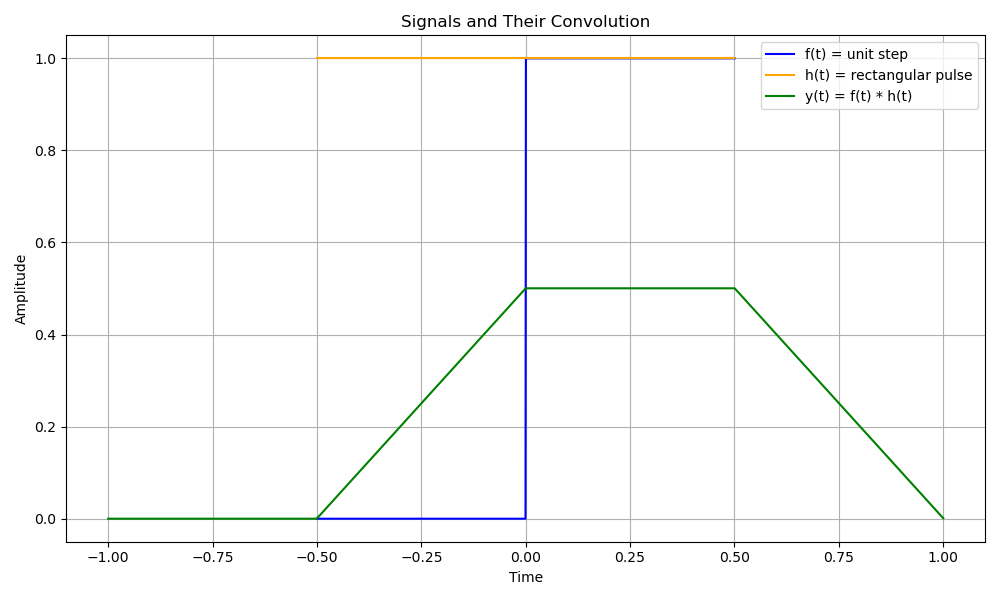
\includegraphics[width=0.6\textwidth]{figs/t_0.5.png}
    \caption{T = 0.5}
    \label{fig:t_0.5.png}
\end{figure}
\begin{figure}[h]
    \centering
    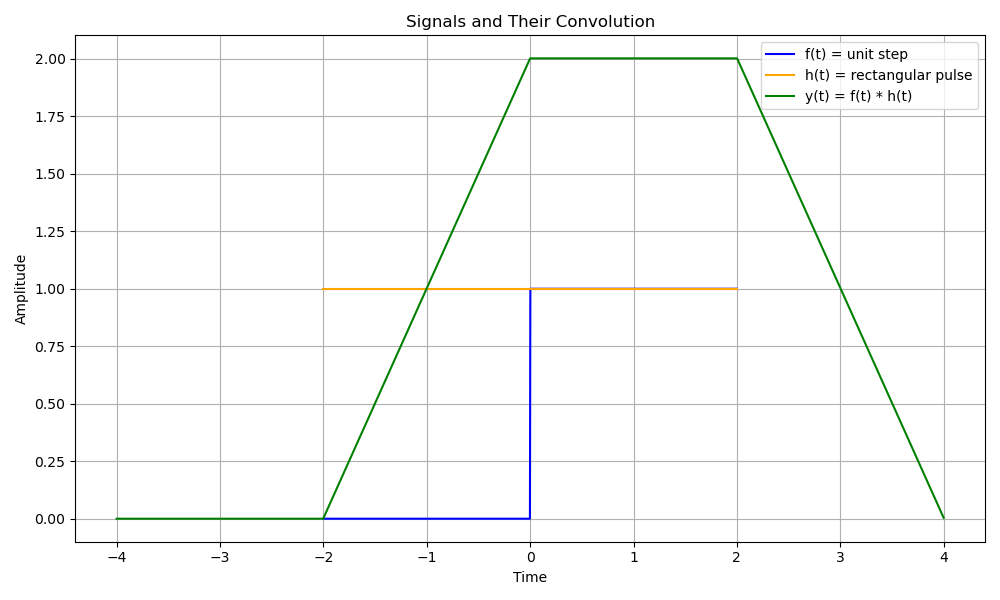
\includegraphics[width=0.6\textwidth]{figs/t_2.png}
    \caption{T = 2}
    \label{fig:conv_sinc}
\end{figure}
\begin{figure}[h]
    \centering
    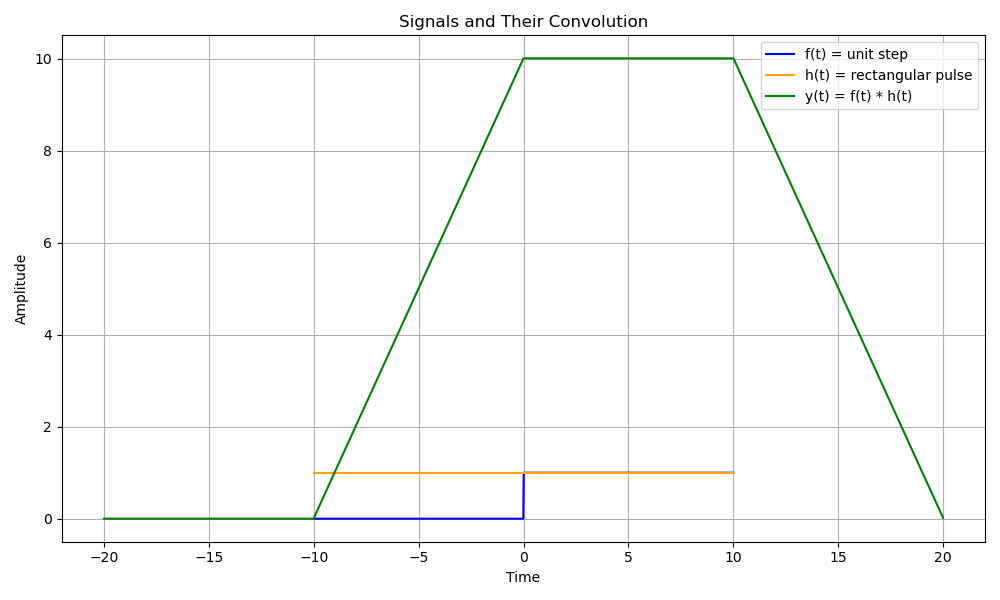
\includegraphics[width=0.6\textwidth]{figs/t_10.png}
    \caption{T = 10}
    \label{fig:conv_sinc}
\end{figure}

\newpage
